\documentclass[tikz,border=2mm]{standalone}
\begin{document}
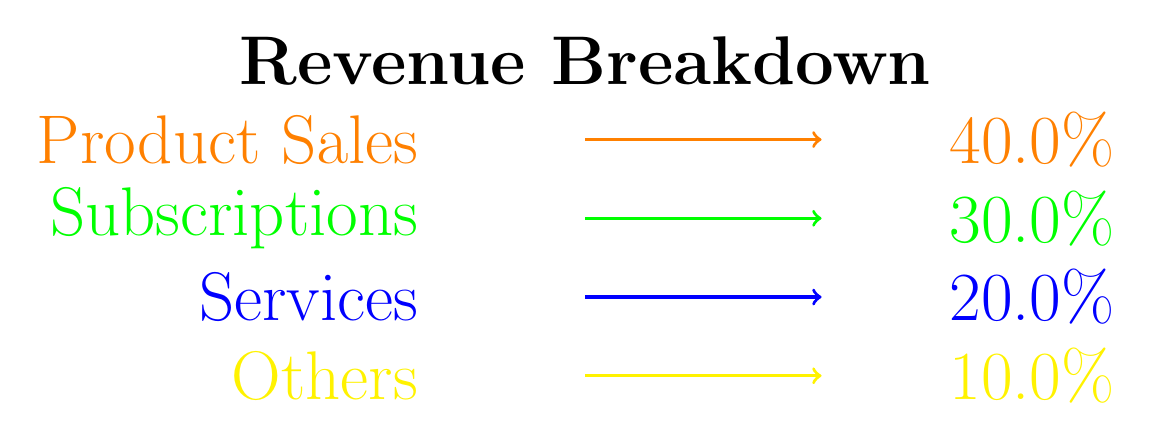
\begin{tikzpicture}

% Title
\node at (0, 5) {\Huge \textbf{Revenue Breakdown}};

% Product Sales
\draw[->, very thick, orange] (0,4) -- (3,4);
\node[anchor=east] at (-2,4) {\Huge \textcolor{orange}{Product Sales}};
\node[anchor=west] at (4.5,4) {\Huge \textcolor{orange}{40.0\%}};

% Subscriptions
\draw[->, very thick, green] (0,3) -- (3,3);
\node[anchor=east] at (-2,3) {\Huge \textcolor{green}{Subscriptions}};
\node[anchor=west] at (4.5,3) {\Huge \textcolor{green}{30.0\%}};

% Services
\draw[->, very thick, blue] (0,2) -- (3,2);
\node[anchor=east] at (-2,2) {\Huge \textcolor{blue}{Services}};
\node[anchor=west] at (4.5,2) {\Huge \textcolor{blue}{20.0\%}};

% Others
\draw[->, very thick, yellow] (0,1) -- (3,1);
\node[anchor=east] at (-2,1) {\Huge \textcolor{yellow}{Others}};
\node[anchor=west] at (4.5,1) {\Huge \textcolor{yellow}{10.0\%}};

\end{tikzpicture}
\end{document}
